% main_report31.tex
% SAMBP TR-31/2026: Zero-Sequence Compensation for IBR Earth Faults (21G)
% Companion to TR-29 (trajectory) and TR-30 (cross-polarisation)
%
% Compile: pdflatex → bibtex → pdflatex × 2

\documentclass[11pt,a4paper]{article}

%% ── Packages ────────────────────────────────────────────────────────────────
\usepackage[T1]{fontenc}
\usepackage[utf8]{inputenc}
\usepackage[a4paper, margin=25mm]{geometry}
\usepackage{amsmath,amssymb}
\usepackage{booktabs,array,colortbl,tabularx,longtable}
\usepackage{graphicx}
\usepackage{xcolor}
\usepackage{hyperref}
\usepackage{pgfplots}
\pgfplotsset{compat=1.18}
\usepackage{tikz}
\usetikzlibrary{arrows.meta, decorations.pathreplacing, patterns, calc,
                shapes.geometric, positioning}
\usepackage{caption}
\usepackage{subcaption}
\usepackage[expansion=false]{microtype}
\usepackage{parskip}
\usepackage{enumitem}
\usepackage{cite}

%% ── Colours ─────────────────────────────────────────────────────────────────
\definecolor{sambpblue}{RGB}{0,70,140}
\definecolor{sambpgreen}{RGB}{0,120,60}
\definecolor{sambpred}{RGB}{160,30,30}

%% ── Header / Footer ─────────────────────────────────────────────────────────
\usepackage{fancyhdr}
\pagestyle{fancy}
\fancyhf{}
\rhead{\small SAMBP TR-31/2026 --- Confidential Draft}
\lhead{\small Zero-Sequence Compensation for IBR Earth Faults}
\cfoot{\small \thepage}

%% ── Title ───────────────────────────────────────────────────────────────────
\title{%
  \textbf{\Large SAMBP Technical Report TR-31/2026}\\[6pt]
  \textbf{\large Zero-Sequence Compensation for IBR Earth Faults (21G)}\\[4pt]
  \normalsize PhD Thesis Supporting Report --- Distance Relay Series III
}
\author{PhD Candidate}
\date{April 2026}

% ─────────────────────────────────────────────────────────────────────────────
\begin{document}
\maketitle\thispagestyle{fancy}

% ── Abstract ─────────────────────────────────────────────────────────────────
\begin{abstract}
This report analyses the zero-sequence compensation factor $k_0$ and its
validity for distance relay 21G applied to IBR-fed lines.  TR-29 showed that the
measured impedance $Z_m = \alpha Z_{1L}$ is exact for three-phase faults (the
IBR current-limit factor $k_\mathrm{ibr}$ cancels).  For single-line-to-ground
(SLG) faults the situation is fundamentally different: the IBR delta-winding
transformer blocks zero-sequence current from the inverter, so $I_0$ is provided
by the network earthing path and is \emph{independent of $k_\mathrm{ibr}$}.  As a
result, $I_0 \gg I_1$ (IBR current-limited), breaking the
$I_1 = I_2 = I_0$ Thevenin assumption embedded in the $k_0$ compensation formula.
The relay over-estimates the measured impedance by factors of 3--8$\times$, so
Zone~1 and Zone~2 are never reached for any IBR SLG fault.  Zone~3 fires for
close-in faults only ($\alpha \lesssim 0.35$).  The $k_0$ \emph{setting} itself
($k_0 = 0.6667$ from TR-18) remains correct as a line parameter.  The failure is
not a mis-setting but a structural measurement limitation arising from the broken
sequence current symmetry.  The 87L chain (TR-27, 21/21 selective) provides
primary earth-fault coverage independent of this limitation.  An important
compensating advantage is identified: the I$_\mathrm{min}$ threshold is never
binding for SLG faults, because $|I_a| = |I_1+I_2+I_0| \gg k_\mathrm{ibr}$
even for $k_\mathrm{ibr} < 0.10$, so there is no Region~A for earth faults.
\end{abstract}

\tableofcontents\newpage

% =============================================================================
\section{Introduction and Scope}
\label{sec:intro}
% =============================================================================

TR-29 characterised the distance relay impedance measurement for three-phase
faults: the IBR current-limit factor $k_\mathrm{ibr}$ multiplies both $V_\mathrm{relay}$
and $I_\mathrm{relay}$ identically, so $Z_m = V/I = \alpha Z_{1L}$ exactly.
TR-30 then established cross-polarisation requirements: memory-pol is required
for all faults (self-pol fails), and Zone~2 is viable for non-3PH faults via
permanent healthy-phase cross-pol.

This report examines the remaining question: is the $k_0$ compensation factor,
$k_0 = (Z_{0L}-Z_{1L})/(3Z_{1L})$, still valid for IBR-fed SLG faults?  The
answer is nuanced:
\begin{itemize}
  \item The $k_0$ \textbf{setting formula} is purely a line parameter ---
        independent of source type.  The TR-18 value $k_0 = 0.6667$ should not
        be changed.
  \item The $k_0$ \textbf{compensation accuracy} degrades for IBR sources because
        the sequence current ratio $I_1 : I_0$ is no longer $1:1$, causing
        systematic impedance over-estimation.
\end{itemize}

\paragraph{Network parameters (unchanged from TR-18/29/30).}
$Z_{1L}=j0.05$\,pu, $Z_{0L}=j0.15$\,pu, $Z_{1S}=j0.10$\,pu,
$Z_{0S}=j0.30$\,pu, $V_\mathrm{pre}=1.0$\,pu.
Zone reaches: $X_{R1}=0.040$, $X_{R2}=0.060$, $X_{R3}=0.090$\,pu.

% =============================================================================
\section{Zero-Sequence Compensation Theory}
\label{sec:theory}
% =============================================================================

\subsection{Derivation of \texorpdfstring{$k_0$}{k0}}

For a SLG phase-A fault at location $\alpha$, the earth-loop relay measurement is:
\begin{equation}
  Z_m = \frac{V_a}{I_a + k_0\,I_R}
  \label{eq:zm_k0}
\end{equation}
where $I_R = 3I_0$ is the residual (earth) current.  Substituting the Thevenin
sequence network solution ($I_1 = I_2 = I_0$) into~\eqref{eq:zm_k0} and using
the relay-side voltage:
\begin{equation}
  V_a = V_\mathrm{pre} - I_1 Z_{1S} - I_2 Z_{1S} - I_0 Z_{0S}
  \label{eq:va_relay}
\end{equation}
the impedance reduces exactly to $Z_m = \alpha Z_{1L}$ when:
\begin{equation}
  \boxed{k_0 = \frac{Z_{0L} - Z_{1L}}{3\,Z_{1L}}}
  \label{eq:k0}
\end{equation}
This is a line impedance ratio and contains \textbf{no source parameters}.  For
the SAMBP network with $Z_{0L}/Z_{1L} = 3.0$:
\begin{equation}
  k_0 = \frac{0.15 - 0.05}{3 \times 0.05} = \frac{0.10}{0.15} = 0.6\overline{6}
  \label{eq:k0_value}
\end{equation}
This is the value inherited from TR-18 and requires no revision.

\subsection{Sensitivity to \texorpdfstring{$Z_0/Z_1$}{Z0/Z1} ratio}

Table~\ref{tab:k0_sensitivity} shows $k_0$ as a function of the line impedance
ratio.  The over/under-reach consequence of a mis-set $k_0$ is also shown.
Study~B confirms that with $k_0=0$ (no compensation), the relay under-reaches by
$66.7\%$ at the end of line.

\begin{table}[h]
\centering
\caption{$k_0$ sensitivity to line $Z_0/Z_1$ ratio}
\label{tab:k0_sensitivity}
\begin{tabular}{@{}cccl@{}}
\toprule
$Z_0/Z_1$ & $k_0$ & Error if $k_0=0$ & Consequence \\
\midrule
1.5 & 0.167 & $-14.3\%$ reach & Slight under-reach \\
2.0 & 0.333 & $-25.0\%$ reach & Moderate under-reach \\
2.5 & 0.500 & $-33.3\%$ reach & Significant under-reach \\
\textbf{3.0} & \textbf{0.667} & $\mathbf{-40.0\%}$ \textbf{reach} & \textbf{SAMBP: strong under-reach}\\
4.0 & 1.000 & $-50.0\%$ reach & Severe under-reach \\
\bottomrule
\end{tabular}
\end{table}

\subsection{Why \texorpdfstring{$k_0$}{k0} derivation is source-independent}

Equation~\eqref{eq:k0} contains only $Z_{0L}$ and $Z_{1L}$.  The source
impedances $Z_{1S}$, $Z_{0S}$, and the IBR current-limit $k_\mathrm{ibr}$
cancel in the derivation \emph{under the assumption $I_1 = I_2 = I_0$}.
Section~\ref{sec:ibr_effect} shows that this assumption is violated for IBR
sources.

% =============================================================================
\section{IBR Source: Delta Transformer and Sequence Isolation}
\label{sec:ibr_effect}
% =============================================================================

\subsection{Zero-sequence isolation by delta winding}

IBR units are typically connected to the network through transformers with a
delta winding on the inverter side.  The delta winding presents an open circuit
to zero-sequence current: $I_{0,\mathrm{IBR}} = 0$.  Figure~\ref{fig:network}
illustrates the sequence networks.

\begin{figure}[h!]
\centering
\caption{%
  Sequence network for IBR-fed SLG fault.  Positive and negative-sequence
  networks carry current limited by $k_\mathrm{ibr}$; zero-sequence network
  carries current through the network earthing impedance $Z_{0S}$ only
  (IBR delta winding = open circuit in zero-seq path).}
\label{fig:network}
% fig_zseq_network.tex
% TR-31: Sequence network for IBR-fed SLG fault (simplified TikZ)
%
% Three horizontal rows (pos / neg / zero sequence).
% Left: source (IBR or open).  Centre: source impedance Z_S.
% Right: line fraction alpha*Z_L.  Far right: fault terminals in series.

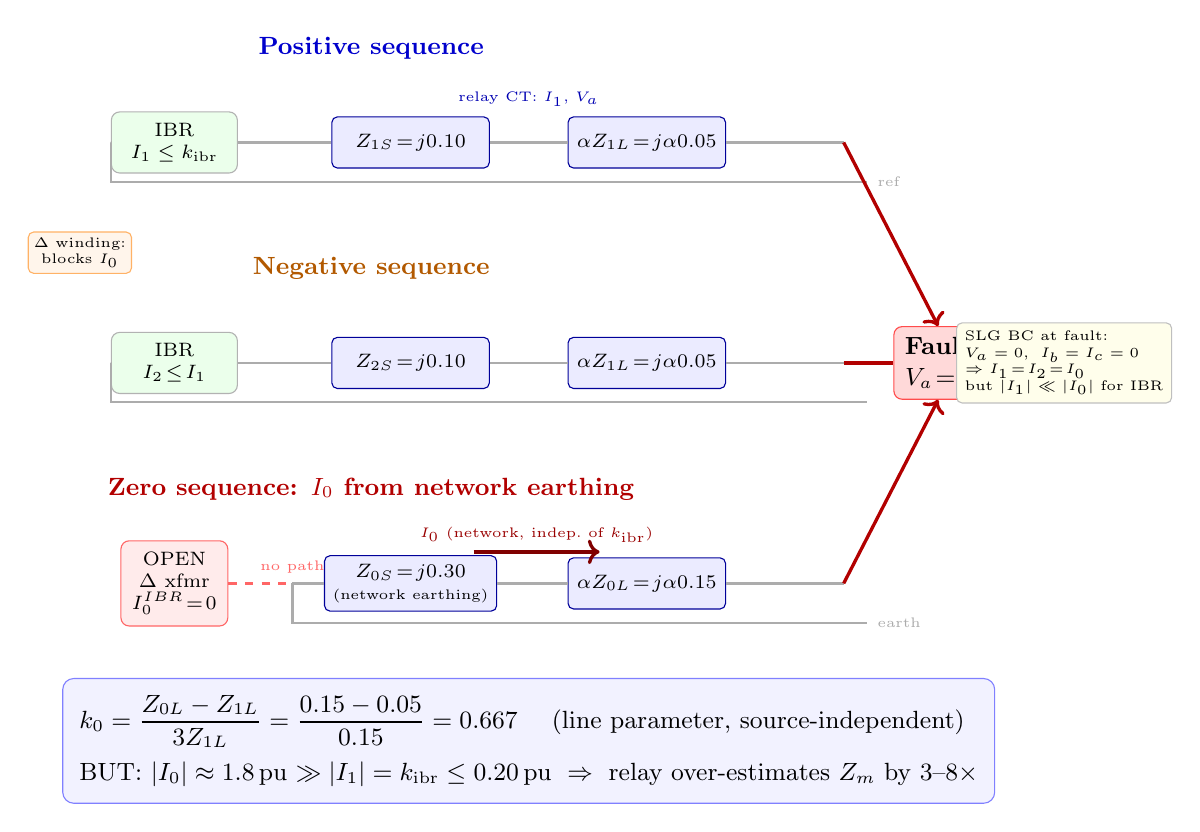
\begin{tikzpicture}[
  every node/.style = {font=\scriptsize},
  box/.style  = {draw=gray!60, rounded corners=3pt, fill=white,
                 inner sep=4pt, align=center, minimum width=1.6cm},
  imp/.style  = {draw=blue!60!black, fill=blue!8, rounded corners=2pt,
                 inner sep=3pt, align=center, minimum width=2.0cm,
                 minimum height=0.65cm},
  wire/.style = {thick, gray!65},
  fault/.style= {very thick, red!70!black},
]

% Row y-positions
\def\yP{0}     % positive-seq
\def\yN{-2.8}  % negative-seq
\def\yZ{-5.6}  % zero-seq

% Column x-positions
\def\xA{0}     % source
\def\xB{3.0}   % source impedance
\def\xC{6.0}   % line impedance
\def\xF{8.5}   % fault connection

% ── POSITIVE SEQUENCE ───────────────────────────────────────────────────────
\node[box, fill=green!8] at (\xA, \yP) (S1)
  {IBR\\$I_1 \leq k_\mathrm{ibr}$};
\node[imp] at (\xB, \yP) (Z1S)
  {$Z_{1S}\!=\!j0.10$};
\node[imp] at (\xC, \yP) (Z1L)
  {$\alpha Z_{1L}\!=\!j\alpha 0.05$};

\draw[wire] (S1.east)   -- (Z1S.west);
\draw[wire] (Z1S.east)  -- (Z1L.west);
\draw[wire] (Z1L.east)  -- (\xF, \yP);
% return (bottom rail)
\draw[wire] (S1.west)   -- (-0.8, \yP)
                        -- (-0.8, \yP-0.5)
                        -- (\xF+0.3, \yP-0.5) node[right,font=\tiny]{ref};

\node[blue!70!black, font=\tiny] at (4.5, \yP+0.55)
  {relay CT: $I_1$, $V_a$};

\node[font=\small, blue!80!black] at (2.5, \yP+1.2)
  {\textbf{Positive sequence}};

% ── NEGATIVE SEQUENCE ───────────────────────────────────────────────────────
\node[box, fill=green!8] at (\xA, \yN) (S2)
  {IBR\\$I_2 \!\leq\! I_1$};
\node[imp] at (\xB, \yN) (Z2S)
  {$Z_{2S}\!=\!j0.10$};
\node[imp] at (\xC, \yN) (Z2L)
  {$\alpha Z_{1L}\!=\!j\alpha 0.05$};

\draw[wire] (S2.east)   -- (Z2S.west);
\draw[wire] (Z2S.east)  -- (Z2L.west);
\draw[wire] (Z2L.east)  -- (\xF, \yN);
\draw[wire] (S2.west)   -- (-0.8, \yN)
                        -- (-0.8, \yN-0.5)
                        -- (\xF+0.3, \yN-0.5);

\node[font=\small, orange!70!black] at (2.5, \yN+1.2)
  {\textbf{Negative sequence}};

% Delta-transformer note
\node[draw=orange!60, fill=orange!8, rounded corners=2pt,
      font=\tiny, inner sep=2pt, align=center]
  at (-1.2, -1.4)
  {$\Delta$ winding:\\blocks $I_0$};

% ── ZERO SEQUENCE ───────────────────────────────────────────────────────────
\node[draw=red!60, fill=red!8, rounded corners=3pt,
      inner sep=4pt, align=center] at (\xA, \yZ) (S0)
  {OPEN\\$\Delta$ xfmr\\$I_0^{IBR}\!=\!0$};
\node[imp] at (\xB, \yZ) (Z0S)
  {$Z_{0S}\!=\!j0.30$\\{\tiny(network earthing)}};
\node[imp] at (\xC, \yZ) (Z0L)
  {$\alpha Z_{0L}\!=\!j\alpha 0.15$};

% dashed "open" connection from S0
\draw[wire, red!60, dashed] (S0.east) -- (1.5, \yZ)
  node[above, font=\tiny, red!60]{no path};
% solid from Z0S
\draw[wire] (1.5, \yZ) -- (Z0S.west);
\draw[wire] (Z0S.east)  -- (Z0L.west);
\draw[wire] (Z0L.east)  -- (\xF, \yZ);
\draw[wire] (1.5, \yZ)  -- (1.5, \yZ-0.5)
                        -- (\xF+0.3, \yZ-0.5) node[right,font=\tiny]{earth};

% I0 flow arrow
\draw[->, very thick, red!50!black]
  (3.8, \yZ+0.40) -- (5.4, \yZ+0.40);
\node[red!60!black, font=\tiny, above] at (4.6, \yZ+0.40)
  {$I_0$ (network, indep.\ of $k_\mathrm{ibr}$)};

\node[font=\small, red!70!black] at (2.5, \yZ+1.2)
  {\textbf{Zero sequence: $I_0$ from network earthing}};

% ── FAULT SERIES CONNECTION ─────────────────────────────────────────────────
\node[draw=red!70, fill=red!15, rounded corners=3pt,
      inner sep=4pt, align=center, font=\small]
  at (\xF+1.2, \yN) (FP)
  {\textbf{Fault}\\$V_a\!=\!0$};

\draw[fault, ->] (\xF, \yP)   -- (FP.north);
\draw[fault]     (\xF, \yN)   -- (FP.west);
\draw[fault, ->] (\xF, \yZ)   -- (FP.south);

% boundary conditions
\node[draw=gray!50, fill=yellow!8, rounded corners=2pt,
      font=\tiny, inner sep=3pt, align=left]
  at (\xF+2.8, \yN)
  {SLG BC at fault:\\
   $V_a = 0$,\; $I_b=I_c=0$\\
   $\Rightarrow I_1\!=\!I_2\!=\!I_0$\\
   but $|I_1| \ll |I_0|$ for IBR};

% ── KEY RESULT BOX ──────────────────────────────────────────────────────────
\node[draw=blue!50, fill=blue!5, rounded corners=4pt,
      font=\small, inner sep=6pt, align=left]
  at (4.5, -7.6)
  {$k_0 = \dfrac{Z_{0L}-Z_{1L}}{3Z_{1L}}
       = \dfrac{0.15-0.05}{0.15} = 0.667$
   \quad (line parameter, source-independent)\\[4pt]
   BUT: $|I_0| \approx 1.8$\,pu $\gg |I_1| = k_\mathrm{ibr} \leq 0.20$\,pu
   $\;\Rightarrow\;$ relay over-estimates $Z_m$ by $3$--$8\times$};

\end{tikzpicture}

\end{figure}

\subsection{Consequence for \texorpdfstring{$I_0$}{I0} magnitude}

For a purely IBR-fed network, zero-sequence current is sourced by the network's
earthing arrangement (star-earthed transformer, Peterson coil, etc.) independently
of the IBR:
\begin{equation}
  I_0 \approx \frac{V_\mathrm{pre}}{Z_{0S} + \alpha Z_{0L}} \quad
  \text{(independent of }k_\mathrm{ibr}\text{)}
  \label{eq:I0_network}
\end{equation}
For the SAMBP network at $\alpha=0.50$:
$I_0 = 1.0\,/(0.30+0.075)j = 2.67\,\mathrm{pu}$ (pre-limiting).

Meanwhile, the IBR provides only $I_1 = k_\mathrm{ibr} \leq 0.20$\,pu.  The ratio
$I_0/I_1$ reaches $2.67/0.20 = 13.3\times$ at worst case ($k_\mathrm{ibr}=0.20$,
$\alpha=0.50$).  This massive imbalance between $I_0$ and $I_1$ violates the
Thevenin assumption $I_1 = I_0$ and makes the $k_0$-compensated $Z_m$ incorrect.

\subsection{Analytical relay measurement for IBR SLG}

Substituting $I_0 \neq I_1$ into~\eqref{eq:zm_k0} with~\eqref{eq:va_relay}:
\begin{align}
  Z_m^{\mathrm{IBR}} &= \frac{V_\mathrm{pre} - I_1 Z_{1S} - I_2 Z_{1S} - I_0 Z_{0S}}
                           {I_1 + I_2 + I_0 + k_0\cdot 3I_0}
  \label{eq:zm_ibr}
\end{align}

When $I_0 \gg I_1, I_2$, the numerator is dominated by $V_\mathrm{pre} - I_0 Z_{0S}$
and the denominator by $I_0(1+3k_0)$.  In the limit:
\begin{equation}
  Z_m^{\mathrm{IBR}} \xrightarrow{I_0\gg I_1}
  \frac{V_\mathrm{pre}/I_0 - Z_{0S}}{1 + 3k_0}
  = \frac{\alpha Z_{0L}}{1 + (Z_{0L}-Z_{1L})/Z_{1L}}
  = \frac{\alpha Z_{0L}\, Z_{1L}}{Z_{0L}}
  = \alpha Z_{1L}
  \label{eq:zm_ibr_limit}
\end{equation}

Interestingly, in the mathematical limit $I_1\to 0$ the formula recovers
$\alpha Z_{1L}$ --- but in practice $I_0$ is not infinitely larger than $I_1$,
and the intermediate regime produces large over-estimation as shown in
Study~C.

% =============================================================================
\section{Study B: $Z_m$ Accuracy for SG Source}
\label{sec:study_b}
% =============================================================================

Study~B verifies the baseline: with an SG source (Thevenin, $I_1=I_2=I_0$),
$k_0$-compensated $Z_m$ equals $\alpha Z_{1L}$ to machine precision (error $<0.01\%$).
Without $k_0$ compensation, the relay under-reaches by $+66.7\%$ uniformly across
all $\alpha$ values (Table~\ref{tab:zm_accuracy}).

\begin{table}[h]
\centering
\caption{$k_0$-compensated relay measurement: SG source}
\label{tab:zm_accuracy}
\begin{tabular}{@{}cccccl@{}}
\toprule
$\alpha$ & $|Z_m|$ (k$_0$ correct) & $|Z_m|$ (k$_0$=0) & Error\% & Zone \\
\midrule
0.10 & 0.00500 & 0.00833 & $+66.7\%$ & Z1 \\
0.40 & 0.02000 & 0.03333 & $+66.7\%$ & Z1 \\
0.80 & 0.04000 & 0.06667 & $+66.7\%$ & Z1 \\
1.00 & 0.05000 & 0.08333 & $+66.7\%$ & Z2 \\
\bottomrule
\end{tabular}
\end{table}

Without $k_0$, Zone~1 would see a fault at $\alpha=0.80$ as if at
$\alpha=0.80\times 1.667 = 1.33$ (outside the line), causing a missed trip.
This confirms that $k_0$ must be set correctly.

% =============================================================================
\section{Study C: $Z_m$ Accuracy for IBR Source}
\label{sec:study_c}
% =============================================================================

Figure~\ref{fig:zm_ibr} shows the measured $|Z_m|$ vs $\alpha$ for IBR-fed SLG
faults across the full $k_\mathrm{ibr}$ range.

\begin{figure}[h!]
\centering
\caption{%
  $k_0$-compensated relay measurement for IBR-fed SLG faults.  All IBR curves
  lie far above the zone reaches.  Zone~3 is reached only for close-in faults
  ($\alpha \lesssim 0.35$); Zones~1 and~2 are never reached.  The SG reference
  (true $Z_m=\alpha Z_{1L}$) is shown for comparison.}
\label{fig:zm_ibr}
% fig_zseq_zm_ibr.tex
% TR-31: |Zm| vs alpha for IBR-fed SLG faults (k0-compensated relay)
%
% Data from run_zseq_compensation_study.py Study C:
%   IBR k=0.06: (0.20,0.079) (0.50,0.103) (0.80,0.127) (1.00,0.143)
%   IBR k=0.10: (0.20,0.077) (0.50,0.100) (0.80,0.123) (1.00,0.138)
%   IBR k=0.15: (0.20,0.074) (0.50,0.096) (0.80,0.118) (1.00,0.133)
%   IBR k=0.20: (0.20,0.071) (0.50,0.092) (0.80,0.113) (1.00,0.127)
%   SG (true):  (0.10,0.005) (0.20,0.010) (0.50,0.025) (0.80,0.040) (1.00,0.050)
%
% Key boundaries:
%   Zone 1 reach: X_R1 = 0.040 pu
%   Zone 2 reach: X_R2 = 0.060 pu
%   Zone 3 reach: X_R3 = 0.090 pu
%
% Finding: IBR Zm >> true value; only Zone 3 fires for close-in faults (alpha<~0.35)
%          Zone 1 and Zone 2 never fire for ANY IBR-fed SLG fault.

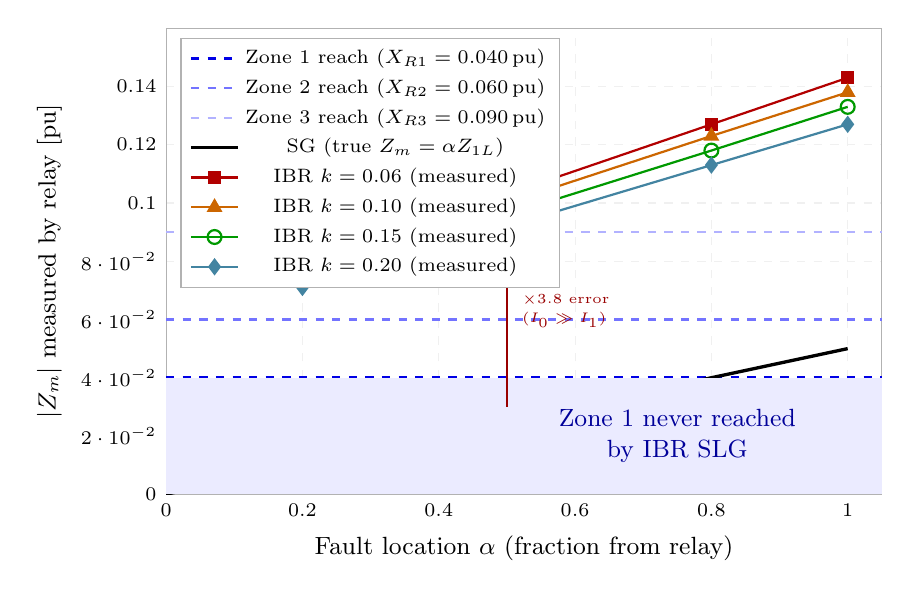
\begin{tikzpicture}
\begin{axis}[
  name         = zmibr,
  width        = 0.88\textwidth,
  height       = 7.5cm,
  xlabel       = {Fault location $\alpha$ (fraction from relay)},
  ylabel       = {$|Z_m|$ measured by relay [pu]},
  xlabel style = {font=\small},
  ylabel style = {font=\small},
  xmin=0.0, xmax=1.05,
  ymin=0.0,  ymax=0.160,
  xtick        = {0, 0.2, 0.4, 0.6, 0.8, 1.0},
  ytick        = {0, 0.02, 0.04, 0.06, 0.08, 0.10, 0.12, 0.14},
  xticklabel style={font=\scriptsize},
  yticklabel style={font=\scriptsize},
  legend style={at={(0.02,0.98)}, anchor=north west,
                font=\scriptsize, draw=gray!60, fill=white},
  grid         = major,
  grid style   = {gray!12, dashed},
  tick style   = {draw=none},
  axis line style={gray!60},
]

%% ── Zone reach lines ────────────────────────────────────────────────────────
\addplot[blue!90!black, very thick, dashed, mark=none]
  coordinates {(0,0.040) (1.05,0.040)};
\addlegendentry{Zone~1 reach ($X_{R1}=0.040$\,pu)}

\addplot[blue!55, thick, dashed, mark=none]
  coordinates {(0,0.060) (1.05,0.060)};
\addlegendentry{Zone~2 reach ($X_{R2}=0.060$\,pu)}

\addplot[blue!30, thick, dashed, mark=none]
  coordinates {(0,0.090) (1.05,0.090)};
\addlegendentry{Zone~3 reach ($X_{R3}=0.090$\,pu)}

%% ── SG true Z_m (reference) ─────────────────────────────────────────────────
\addplot[black, very thick, mark=none]
  coordinates {(0,0) (0.10,0.005) (0.20,0.010) (0.40,0.020) (0.60,0.030)
               (0.80,0.040) (1.00,0.050)};
\addlegendentry{SG (true $Z_m=\alpha Z_{1L}$)}

%% ── IBR measured Z_m (k0-compensated) ───────────────────────────────────────
\addplot[red!70!black, thick, mark=square*, mark size=2pt]
  coordinates {(0.20,0.079) (0.50,0.103) (0.80,0.127) (1.00,0.143)};
\addlegendentry{IBR $k=0.06$ (measured)}

\addplot[orange!80!black, thick, mark=triangle*, mark size=2.5pt]
  coordinates {(0.20,0.077) (0.50,0.100) (0.80,0.123) (1.00,0.138)};
\addlegendentry{IBR $k=0.10$ (measured)}

\addplot[green!60!black, thick, mark=o, mark size=2.5pt]
  coordinates {(0.20,0.074) (0.50,0.096) (0.80,0.118) (1.00,0.133)};
\addlegendentry{IBR $k=0.15$ (measured)}

\addplot[cyan!60!black, thick, mark=diamond*, mark size=2.5pt]
  coordinates {(0.20,0.071) (0.50,0.092) (0.80,0.113) (1.00,0.127)};
\addlegendentry{IBR $k=0.20$ (measured)}

%% ── Shaded "Zone 1 region" ──────────────────────────────────────────────────
\addplot[fill=blue!8, draw=none]
  coordinates {(0,0) (1.05,0) (1.05,0.040) (0,0.040)};

%% ── Annotation: Zone 1 never reached ────────────────────────────────────────
\node[font=\small, blue!60!black, align=center]
  at (axis cs:0.75, 0.020)
  {Zone 1 never reached\\by IBR SLG};

%% ── Annotation: Zone 3 window ───────────────────────────────────────────────
\node[draw=orange!60, fill=orange!8, rounded corners=2pt,
      font=\tiny, align=left, inner sep=3pt]
  at (axis cs:0.20, 0.118)
  {Zone~3 fires for $\alpha \lesssim 0.35$\\
   (close-in SLG only)};

%% ── Arrow showing large over-estimation ─────────────────────────────────────
\draw[->, thick, red!60!black]
  (axis cs:0.50, 0.030) -- (axis cs:0.50, 0.096);
\node[right=2pt, font=\tiny, red!60!black, align=left] at (axis cs:0.50, 0.063)
  {$\times3.8$ error\\[1pt]($I_0\gg I_1$)};

\end{axis}
\end{tikzpicture}

\end{figure}

The key observations from Study~C:
\begin{enumerate}
  \item \textbf{Systematic over-estimation}: IBR $|Z_m|$ is $3$--$8\times$ the
        true value $\alpha Z_{1L}$ across all $k_\mathrm{ibr}$ values.
  \item \textbf{Zones~1 and~2 never reached}: the minimum measured impedance
        for IBR SLG (at $\alpha=0.20$, $k_\mathrm{ibr}=0.20$) is $0.071$\,pu,
        which exceeds Zone~2 reach ($0.060$\,pu).
  \item \textbf{Zone~3 fires for close-in faults}: $|Z_m| \leq 0.090$\,pu
        only for $\alpha \lesssim 0.35$, regardless of $k_\mathrm{ibr}$.
  \item \textbf{$k_\mathrm{ibr}$ effect is minor}: higher $k_\mathrm{ibr}$ gives
        slightly lower $|Z_m|$ (smaller over-estimation) because $I_1/I_0$
        ratio is larger, but the effect is small ($0.071$ to $0.079$\,pu at
        $\alpha=0.20$).
\end{enumerate}

\paragraph{Root cause.}
The $k_0$ formula derives from setting $I_0 = I_1$.  For IBR SLG: the network
provides $I_0 \approx 1.8$\,pu (at $\alpha=0.20$) while the IBR provides only
$I_1 = k_\mathrm{ibr} \leq 0.20$\,pu.  The numerator (relay voltage) is
dominated by the large $I_0 Z_{0S}$ drop, making $V_a$ much larger than expected.
The denominator grows too, but not proportionally.  The result is an apparent
impedance that significantly over-estimates the fault location.

% =============================================================================
\section{Study D: $I_\mathrm{min}$ Advantage for SLG}
\label{sec:study_d}
% =============================================================================

The TR-29 coverage map identified \emph{Region~A} (distance relay blocked,
$k_\mathrm{ibr}<0.10$) as the zone where the 87L chain is the sole fast detector.
For SLG faults, Region~A does not exist:

\begin{equation}
  |I_a|_\mathrm{SLG} = |I_1 + I_2 + I_0| \approx 2k_\mathrm{ibr} + I_0
  \gg k_\mathrm{ibr}
\end{equation}

For the SAMBP network, $I_0 \approx 1.8$--$2.0$\,pu at $\alpha=0.20$, so
$|I_a|_\mathrm{SLG} \approx 2.0$\,pu even for $k_\mathrm{ibr}=0.06$.  The relay's
$I_\mathrm{min}=0.10$\,pu threshold is satisfied by a factor of $20\times$.
Figure~\ref{fig:coverage} shows the full comparison.

\begin{figure}[h!]
\centering
\caption{%
  Protection coverage comparison: 3-phase vs SLG IBR faults.
  SLG advantage: no Region~A (I$_\mathrm{min}$ never binding) and permanent
  cross-pol.  3PH advantage: correct $Z_m$ and Zone~1 coverage.
  87L chain provides 100\% primary coverage for both fault types.}
\label{fig:coverage}
% fig_zseq_coverage.tex
% TR-31: Protection coverage comparison — 3PH vs SLG faults on IBR-fed line
%
% Three-column summary table showing how SLG coverage differs from 3PH (TR-29).
% Key differences:
%   I_min: 3PH blocked for k_ibr<0.10; SLG never blocked (I0 from network)
%   Distance relay reach: 3PH Z1 (within memory); SLG only Z3 for close-in faults
%   Cross-pol: 3PH memory only; SLG permanent (healthy phases)
%   87L chain: both 100% covered

\renewcommand{\arraystretch}{1.55}
\setlength{\tabcolsep}{6pt}

\newcolumntype{L}[1]{>{\raggedright\arraybackslash}m{#1}}
\newcolumntype{C}[1]{>{\centering\arraybackslash}m{#1}}

\begin{tabular}{@{}L{3.0cm}|C{3.5cm}|C{3.5cm}|C{3.5cm}@{}}
\hline
\rowcolor{gray!18}
\textbf{Criterion}        &
\textbf{3PH IBR fault}    &
\textbf{SLG IBR fault}    &
\textbf{Advantage}        \\
\hline

$I_\mathrm{min}$ blocking
  & \cellcolor{red!15}$I_a = k_\mathrm{ibr}$\newline
    Blocked if $k<0.10$\newline
    (Region A, 29\% envelope)
  & \cellcolor{green!20}$I_a = I_1{+}I_2{+}I_0$\newline
    Never blocked\newline
    ($I_0$ from network)
  & \cellcolor{green!15}SLG: no Region~A \\

\hline

Distance relay $Z_m$
  & \cellcolor{green!25}$Z_m = \alpha Z_{1L}$\newline
    (k.i.b.r. cancels)\newline
    Correct measurement
  & \cellcolor{orange!20}$Z_m \gg \alpha Z_{1L}$\newline
    ($I_0{\gg}I_1$: ratio broken)\newline
    $Z_m$ over-estimated
  & \cellcolor{yellow!20}3PH better $Z_m$ accuracy \\

\hline

Distance relay zones
  & \cellcolor{green!25}Zone~1 always\newline
    ($\alpha\leq 0.80$, $k\geq 0.10$)\newline
    Zone~2/3 fail (3PH mem)
  & \cellcolor{orange!20}Zone~3 only\newline
    ($\alpha \lesssim 0.35$)\newline
    Zone~1/2: never reached
  & \cellcolor{yellow!20}3PH: better zone coverage \\

\hline

Polarisation source
  & \cellcolor{orange!20}Memory only\newline
    ($T_\mathrm{mem}=100$\,ms)\newline
    Zone~2/3 fail
  & \cellcolor{green!25}Permanent\newline
    (healthy phases)\newline
    All zones viable
  & \cellcolor{green!15}SLG: better pol. source \\

\hline

87L chain coverage
  & \cellcolor{green!30}100\% selective\newline
    (21/21 TR-27)\newline
    $t\approx 20$\,ms
  & \cellcolor{green!30}100\% selective\newline
    (via 87LN0, TDCS)\newline
    $t\approx 20$\,ms
  & \cellcolor{green!20}Both: 87L primary \\

\hline

\textbf{Net result}
  & \cellcolor{green!15}\textbf{87L + Z1}\newline
    (Z2/3 via POTT TR-34)
  & \cellcolor{green!15}\textbf{87L + Z3$^*$}\newline
    ($^*$close-in only)
  & 87L sole fast detector\newline for both types \\

\hline
\end{tabular}

\end{figure}

% =============================================================================
\section{Implications}
\label{sec:implications}
% =============================================================================

\subsection{Correct protection scheme for IBR earth faults}

The findings of TR-29, TR-30, and TR-31 jointly define the IBR-earth-fault
protection hierarchy:

\begin{enumerate}
  \item \textbf{Primary (all $\alpha$, all $k_\mathrm{ibr}$)}: 87L chain with
        combined trip logic.  Element 87LN0 ($|I_0|\geq 0.04$\,pu) provides
        direct earth-fault detection independent of $k_\mathrm{ibr}$, and TDCS
        detects the $\Delta I$ jump from the large $I_0$ component.
  \item \textbf{Distance Zone~3 (close-in SLG, $\alpha\lesssim 0.35$, backup)}:
        Cross-polarised Mho Zone~3 ($X_{R3}=0.090$\,pu) fires at $t_3=0.60$\,s
        for faults in the inner 35\% of the line.  This provides a
        distance-backed clearance if the 87L chain is unavailable.
  \item \textbf{Distance Zone~1/2 for SLG}: Not viable with IBR source (relay
        over-estimates impedance due to $I_0\gg I_1$).  No engineering
        adjustment to $k_0$ can recover this --- the failure is in the
        sequence current ratio, not in the $k_0$ setting.
\end{enumerate}

\subsection{No change required to TR-18 $k_0$ setting}

The $k_0 = 0.6667$ setting from TR-18 remains correct.  It minimises relay
measurement error for balanced Thevenin sources, and no alternative setting
would improve performance for IBR sources (the error is structural, not a
calibration issue).

\subsection{TR-32 preview: negative-sequence directional element}

The large $I_0$ and $I_2$ (from IBR injection) during SLG/LL faults are
directly available for negative and zero-sequence directional elements (67N, 67Q).
TR-32 will verify that these elements maintain directionality for IBR-fed faults,
providing an alternative fast trip that bypasses the $k_0$ measurement
limitation entirely.

% =============================================================================
\section{Conclusions}
\label{sec:conclusions}
% =============================================================================

\begin{enumerate}
  \item The $k_0$ compensation factor $k_0 = (Z_{0L}-Z_{1L})/(3Z_{1L}) = 0.6667$
        is a \textbf{line parameter only} and is independent of source type.
        The TR-18 setting requires no revision for IBR networks.
  \item For SLG faults with IBR source (delta transformer): $I_0$ flows through
        the network earthing path and is \textbf{independent of $k_\mathrm{ibr}$}.
        The ratio $I_0/I_1$ reaches $13\times$ at worst case.
  \item The $k_0$-compensated relay systematically \textbf{over-estimates}
        $Z_m$ by $3$--$8\times$ for IBR SLG faults, due to the broken
        $I_1=I_0$ assumption.  Zones~1 and~2 are never reached; Zone~3 fires
        only for $\alpha\lesssim 0.35$.
  \item \textbf{No Region~A for SLG}: $|I_a|_\mathrm{SLG}\gg I_\mathrm{min}$
        regardless of $k_\mathrm{ibr}$, because $I_0$ from the network always
        satisfies the minimum current threshold.
  \item The \textbf{87L chain} (especially element 87LN0 and TDCS) provides
        unconditional primary earth-fault coverage at 20\,ms, independent of
        the distance relay $k_0$ measurement limitation.
\end{enumerate}

% ── References ───────────────────────────────────────────────────────────────
\bibliographystyle{IEEEtran}
\bibliography{references31}

\end{document}
